\section{Improving Premise Selection of Theorem-Proving Agents}
\subsection{Introduction}
Automated theorem proving and AI-assisted mathematical reasoning depend on premise selection: given a target theorem, the system must find earlier lemmas and theorems that can be used in its proof. The quality of these premises largely determines the size of the proof search problem. A relevant lemma can reduce a difficult goal to a known argument; an irrelevant neighbor increases the number of proof paths the system must consider. The main difficulty is that semantic similarity is only a proxy for logical dependence. A theorem is often close in embedding space to statements about the same objects, notation, or topic. Its proof, however, may cite earlier results that introduce a tool, a reduction, a classification theorem, or a structural fact whose statement is semantically distinct from the target. A semantic search system can therefore retrieve plausible mathematical neighbors while missing the premises that a proof actually uses.

This experiment examines premise selection in a custom environment that wraps TheoremSearch \cite{theoremsearch2026}. TheoremSearch ranks statements by similarity to a natural-language query, but it does not itself learn which query phrasings are likely to retrieve dependencies. We frame query generation as a sequential decision problem: Given a target theorem, an agent issues a fixed number of natural-language queries, observes the results, and is rewarded for retrieving true dependencies.

This motivates the question of whether reinforcement learning can teach a language model to use semantic search in a way that respects dependency structure. Our results are mixed: training improves the base Qwen3-8B policy, but performance plateaus below that of frontier models such as Gemini 3.1 Pro and GPT-5.5. Inspection of the learned queries indicates that the policy can formulate coherent, mathematically precise searches but generally lacks the detailed knowledge of the literature required to recognize and retrieve the cited result. A simple expansion over the citation graph recovers substantially more dependencies, suggesting that much of the remaining signal is encoded in the corpus’s graph structure rather than in embedding-based similarity alone.

\subsection{Methodology}
We formulate premise selection as an MDP over the TheoremSearch API. The state contains the target theorem, represented by its natural-language slogan and \LaTeX\ body, together with the set of statements returned by previous queries. The action is a query string passed to a TheoremSearch API call, which returns the top-$k$ statements by cosine similarity over Qwen3-Embedding-8B slogan embeddings \cite{zhang2025qwen3embedding}. The agent may issue at most $H$ queries. The reward gives $+1$ for each newly retrieved true dependency, applies a false-positive penalty $-\alpha$, and gives a terminal bonus proportional to final dependency recall.

The policy is a Qwen3 language model trained to generate query strings conditioned on the current state. We evaluate dependency recall at $k{=}10$ over $H{=}6$ queries. We use the same configuration for the prompted GPT-5.5 and Gemini-3.1-Pro baselines, so comparisons isolate the effect of the query policy rather than the retrieval budget. At each turn, the policy emits a short reasoning trace before the query. This matches the prompted baselines and, empirically, accounts for a substantial part of the improvement over the base model.

\paragraph{Self-distillation objective.} The retrieval reward is sparse and non-differentiable: most sampled query sequences retrieve no true dependencies, and the reward cannot directly supervise individual query tokens. We therefore train the agent using Self-Distillation Policy Optimization (SDPO) \cite{hubotter2026sdpo}, which uses the best rollout from a sampled group as a feedback signal for policy improvement. For each target theorem, we sample $G{=}4$ rollouts. We select the rollout with the highest dependency recall and use its query strings as feedback $f$. The student policy is then trained to match a feedback-conditioned teacher policy without receiving that feedback at inference time. The per-token loss is a symmetric Jensen--Shannon divergence over the generated completion:
\[
	\mathcal{L}_{\text{SDPO}}(\theta)=\sum_t \mathrm{JS}\!\left(\pi_\theta(\cdot\mid x,y_{<t})\,\|\,
	\mathrm{sg}\,\pi_{\text{teacher}}(\cdot\mid x,f,y_{<t})\right).
\]
The teacher is an exponential moving average of the LoRA weights with $\alpha_{\text{EMA}}{=}0.01$, and $\mathrm{sg}$ denotes stop-gradient. The feedback is the agent's own highest-recall query sequence from the sampled group, rather than the ground-truth dependency list. We additionally evaluate a hybrid SDPO+GRPO objective. SDPO trains the policy to imitate the
highest-reward rollout within a sampled group, while GRPO directly optimizes expected reward using group-relative advantages. The hybrid objective optimizes the sum of the SDPO imitation loss and the GRPO policy-gradient loss:
\[
L_{\text{hybrid}}(\theta)
=
L_{\text{SDPO}}(\theta)
+
\lambda L_{\text{GRPO}}(\theta),
\]
with $\lambda \in [0,1]$. For our test, we used $\lambda = 0.5$.

\paragraph{Training and evaluation context.} During sampled training rollouts, the agent sees a compact rendering of each retrieved statement: the slogan (a natural-language summary of the statement), the paper title, the first author, and the citation count. This lets the policy condition later queries on earlier results. However, in greedy evaluation, including retrieved results lowers recall. The longer context shifts the model toward commenting on previous outputs rather than producing a sharper next query. The final reported policy is therefore trained with result context but evaluated without it. All trained policies are LoRA adapters of rank 16 on Qwen3-8B, which update about 0.53\% of the model parameters.

\paragraph{Citation-graph expansion.} TheoremSearch can also return a statement's one-hop dependency neighborhood; i.e., all results that are one dependency edge away from the target. Since premise selection is defined by citation-derived dependencies, we test whether retrieved statements can serve as seeds for graph expansion. After the policy retrieves statements with embedding search, we add the cross-paper one-hop graph neighbors of those statements to the candidate set. We never expand the target statement itself. To prevent data leakage, we also remove any statement from the target's own paper before computing recall. This prevents the evaluation from rewarding a shortcut in which the system copies citations from sibling theorems in the same paper.

\subsection{Related work}
Premise selection is usually studied inside proof-assistant libraries, where a retriever supplies candidate premises to a prover. LeanDojo retrieves premises for Lean proofs \cite{leandojo}, LeanSearch provides semantic search over Mathlib \cite{leansearch-v1, leansearch-v2}, and earlier work trains language models to generate proofs directly \cite{polu2020generative}. This project differs in two ways. First, retrieval itself is the task: the agent is evaluated on whether it recovers dependency edges, not on whether a downstream prover succeeds. Second, the search space is a broad mathematical corpus indexed by dense slogan embeddings, closer to dense-passage retrieval \cite{karpukhin2020dpr,zhang2025qwen3embedding} than to a single formal library.

The learning setup is related to RL-based agentic search, in which a language model learns to interact with a search environment through multi-step interactions \cite{lin2025agenticsearch}. We train with SDPO as the objective \cite{hubotter2026sdpo} because it has been shown to improve sample efficiency and accuracy over strong RLVR baselines \cite{hubotter2026sdpo}. The graph-augmentation experiment is also related to work showing that language models can benefit from explicit graph structure \cite{guo2025g1,zhang2025generalizable}. In this report, the graph is not learned by the model; it is used at retrieval time to expose dependency edges adjacent to the statements the model already retrieves.

\subsection{Results}
\label{sec:results}

\begin{table}[h]
	\centering
	\caption{Dependency recall at ($k{=}10$, $H{=}6$).}
	\label{tab:main}
	\begin{tabular}{lccl}
		\toprule
		System                                         & Recall         & Mean \# of retrieved candidates                     \\
		\midrule
		Qwen3-8B base                                  & $\sim$0.04    & $\sim$60     \\
		Qwen3-8B SDPO                          & 0.079          & $\sim$60  \\
		\quad + cross-paper graph augmentation\  & \textbf{0.134} & $\sim$115 \\
		\quad + same-paper graph augmentation                  & 0.227          & $\sim$140   \\
		\midrule
		Gemini 3.1 Pro                     & 0.170          & $\sim$60           \\
		GPT-5.5                            & 0.264          & $\sim$60        \\
		\bottomrule
	\end{tabular}
\end{table}

\paragraph{Policy improvement saturation.} Figure~\ref{fig:traj} shows validation recall during SDPO training. The untrained Qwen3-8B policy retrieves, on average, 4\% of a target's true dependencies. Adding a short reasoning trace and training with SDPO raises recall to 7.9\%. After that point, further optimization did not meaningfully improve the result. A learning rate of $10^{-6}$ reaches 7.9\%, while $5{\times}10^{-6}$ reaches 7.7\%. Increasing the training set from 1{,}000 to 5{,}060 targets lowers recall to 5.8\%. These results place all trained policies in the same roughly 6--8\% band.

\begin{figure}[h]
	\centering
	\begin{minipage}{0.49\textwidth}
		\centering
		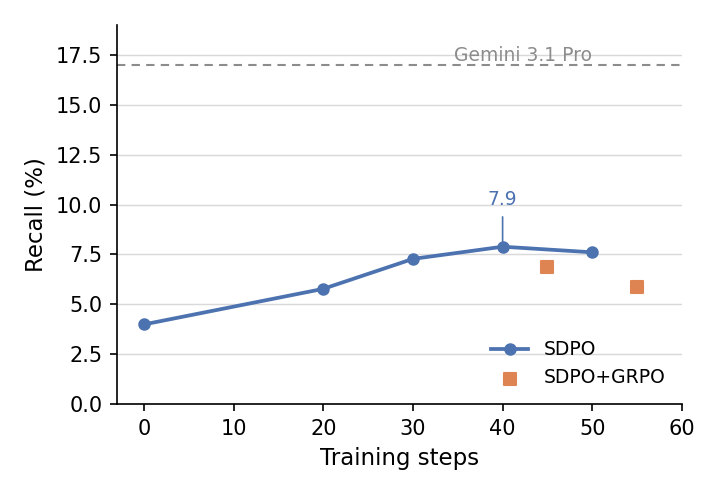
\includegraphics[width=\linewidth]{figures/fig_trajectory.png}
		\caption{Validation recall ($k{=}10$, $H{=}6$) over SDPO training. Recall rises above the base model and then flattens near 8\%, below the prompted Gemini baseline.}
		\label{fig:traj}
	\end{minipage}\hfill
	\begin{minipage}{0.49\textwidth}
		\centering
		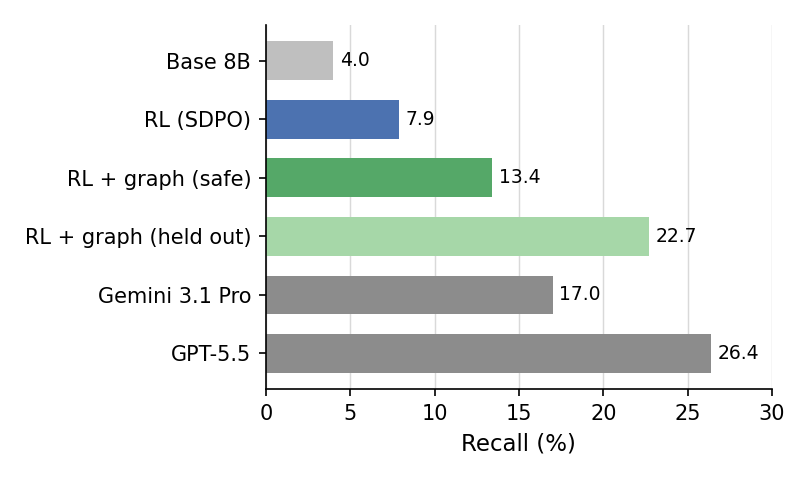
\includegraphics[width=\linewidth]{figures/fig_systems.png}
		\caption{Recall at $k{=}10$. Cross-paper graph expansion roughly doubles the trained policy's recall.}
		\label{fig:systems}
	\end{minipage}
\end{figure}

\paragraph{Citation-graph expansion recovers dependencies that embedding search misses.} Cross-paper graph expansion raises recall from 7.9\% to 13.4\% (Table~\ref{tab:main} and Figure~\ref{fig:systems}). This is because the policy often retrieves a statement near the target, and that nearby statement may cite some of the same background results as the target. One graph hop can therefore turn a semantic near miss into a true dependency. This change closes most of the gap to Gemini-3.1-Pro, although it also increases the candidate set from roughly 60 statements to roughly 115, so the comparison is not on an equal-budget basis. The same-paper expansion reaches 22.7\%, but this is not a valid result for premise selection. Theorems in the same paper share references and often have overlapping dependency lists. Allowing expansion through same-paper siblings therefore lets the method recover citations from the structure of the evaluation set rather than from a dependency-aware query strategy. For this reason, the cross-paper number is the main graph result.

\begin{figure}[h]
	\centering
	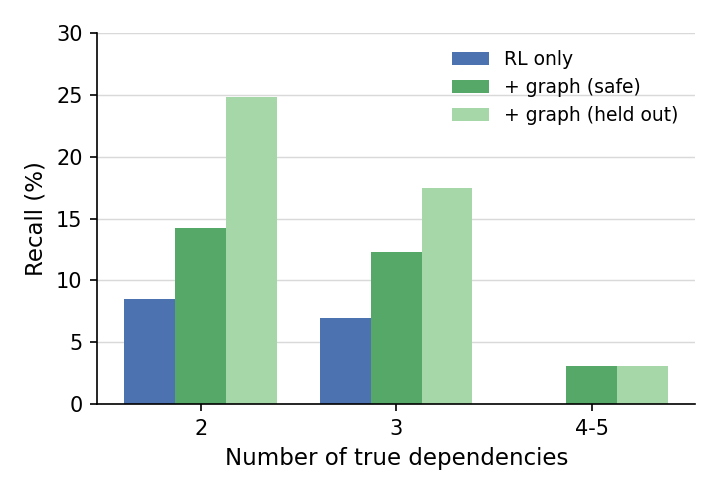
\includegraphics[width=0.5\linewidth]{figures/fig_buckets.png}
	\caption{Recall at $k{=}10$ by number of true dependencies. Cross-paper graph expansion is most effective for low-degree targets.}
	\label{fig:buckets}
\end{figure}

\subsection{Discussion}

\paragraph{Query precision.} The prompted GPT-5.5 and Gemini-3.1-Pro baselines use the same embedding index and a comparable query budget, but retrieve more true dependencies than the trained Qwen3 policy. The trained policy also uses its budget and avoids repeated queries, so the main failure mode is not search control. Instead, it issues mathematically plausible topic queries that rarely name or characterize the exact earlier theorem cited by the proof. This also explains the negative ablations: more data provide little additional signal when most rollout groups contain no successful retrieval.

\paragraph{Graph expansion exposes useful structure.} Cross-paper expansion improves recall because a retrieved statement can be useful even when it is not itself a dependency: if it is close in the citation graph, its own dependencies may overlap with the target's. The gain is largest for low-degree targets, where a few good seeds can cover much of the dependency set (Figure~\ref{fig:buckets}). The same-paper diagnostic shows why this must be evaluated carefully. Same-paper expansion reaches 22.7\%, but that gain comes from shared bibliographies and local paper structure, so it is reported only as leakage.

\paragraph{Limitations.} Differences within the 6--8\% validation band should be treated cautiously because the trained-policy validation set has only $n{=}150$. However, cross-paper graph expansion adds another 5.5 points, which appears to be the more significant statistic. The graph result also uses a larger candidate set, increasing retrieval from roughly 60 to roughly 115 statements, so future systems should pair expansion with re-ranking.

\subsection{Conclusion}
Reinforcement learning improves a Qwen3-8B query policy for premise selection from roughly 4\% to 7.9\% dependency recall at $k{=}10$ under a six-query budget. The improvement then saturates across learning rates and training data scales. This suggests the limiting factor is query precision: the policy learns plausible mathematical searches, but it rarely identifies the exact prior theorem that the target proof cites. Cross-paper citation-graph expansion raises recall to 13.4\% by using retrieved statements as hints for dependency traversal. Future work should focus on learned graph expansion, re-ranking expanded candidates to control budget, and training policies that decide which retrieved statements are worth expanding.